%%%%%%%%%%%%%%%%%%%%%%%%%%%%%%%%%%%%%%%%%
% Frequently Asked Questions
% LaTeX Template
% Version 1.0 (22/7/13)
%
% This template has been downloaded from:
% http://www.LaTeXTemplates.com
%
% Original author:
% Adam Glesser (adamglesser@gmail.com)
%
% License:
% CC BY-NC-SA 3.0 (http://creativecommons.org/licenses/by-nc-sa/3.0/)
%
%%%%%%%%%%%%%%%%%%%%%%%%%%%%%%%%%%%%%%%%%

\documentclass[11pt]{article}

\usepackage[margin=1in]{geometry} % Required to make the margins smaller to fit more content on each page
\usepackage[linkcolor=blue]{hyperref} % Required to create hyperlinks to questions from elsewhere in the document
\hypersetup{pdfborder={0 0 0}, colorlinks=true, urlcolor=blue} % Specify a color for hyperlinks
\usepackage{todonotes} % Required for the boxes that questions appear in
\usepackage{tocloft} % Required to give customize the table of contents to display questions
\usepackage{microtype} % Slightly tweak font spacing for aesthetics
\usepackage{palatino} % Use the Palatino font

\usepackage[utf8x]{inputenc}
\usepackage{sidecap}

\setlength\parindent{0pt} % Removes all indentation from paragraphs

% Create and define the list of questions
\newlistof{questions}{faq}{\large Sections} % This creates a new table of contents-like environment that will output a file with extension .faq
\setlength\cftbeforefaqtitleskip{4em} % Adjusts the vertical space between the title and subtitle
\setlength\cftafterfaqtitleskip{1em} % Adjusts the vertical space between the subtitle and the first question
\setlength\cftparskip{.3em} % Adjusts the vertical space between questions in the list of questions

% Create the command used for questions
\newcommand{\question}[1] % This is what you will use to create a new question
{
\refstepcounter{questions} % Increases the questions counter, this can be referenced anywhere with \thequestions
%\par\noindent % Creates a new unindented paragraph
\phantomsection % Needed for hyperref compatibility with the \addcontensline command
\addcontentsline{faq}{questions}{#1} % Adds the question to the list of questions
\todo[inline, color=green!40]{\textbf{#1}} % Uses the todonotes package to create a fancy box to put the question
\vspace{1em} % White space after the question before the start of the answer
}

% Uncomment the line below to get rid of the trailing dots in the table of contents
\renewcommand{\cftdot}{}

% Uncomment the two lines below to get rid of the numbers in the table of contents
%\let\Contentsline\contentsline
%\renewcommand\contentsline[3]{\Contentsline{#1}{#2}{}}


\ifdefined\frenchmanual
  \newcommand\mtext[2]{#1}
\else
  \newcommand\mtext[2]{#2}
\fi



\begin{document}

%----------------------------------------------------------------------------------------
%	TITLE
%----------------------------------------------------------------------------------------


\begin{flushright}
  \includegraphics[width=0.1\textwidth]{bretagne_quadri.pdf}
\end{flushright}

\begin{center}
\Huge{\bf \emph{\mtext{Wi2Me Recherche - Manuel d'utilisation}{Wi2Me Research - User Manual}}} % Main title
\end{center}

\begin{flushleft}
\todo[inline, color=green!40]{\textbf{\mtext{Introduction et Contact}{Introduction and Contact}}} % Uses the todonotes package to create a fancy box to put the question
\mtext{Ce document présente l'utilisation de l'application de mesure Wi2Me Recherche développée par TELECOM Bretagne. Pour plus d'information ou de support :}{This Document presents the steps required to perform mesurements using the Wi2Me Research application developed by TELECOM Bretagne. For more information or support, feel free to contact : }

Tanguy Kerdoncuff \\ 
tanguy.kerdoncuff@telecom-bretagne.eu\\
+332 99 12 70 49 \\
TELECOM Bretagne - Dept. RSM\\
2, Rue de la Chataigneraie \\
35100 Cesson Sévigné\\
\end{flushleft}

\listofquestions % This prints the subtitle and a list of all of your questions

%\newpage % Comment this if you would like your questions and answers to start immediately after table of questions

%----------------------------------------------------------------------------------------
\question{\mtext{Lancer Wi2Me}{Starting Wi2Me}}\label{starting}

\begin{SCfigure}[\sidecaptionrelwidth][!h]
  \centering
  \caption{ \mtext{Lancer l'application en pressant sur l'icône Wi2Me Research du bureau.}{Start the application by pressing the Wi2Me Research application on the desktop.}}
  \includegraphics[height=0.4\textheight]{open.png}
\end{SCfigure}

\begin{SCfigure}[\sidecaptionrelwidth][!h]
  \centering
  \caption{ \mtext{Ouvrir le menu de wi2me en utilisant le button en bas à gauche (ou le bouton menu physique s'il existe).}{Open the application menu by using the menu button in the bottom left (or your phone's physical menu button if it exists).}}
  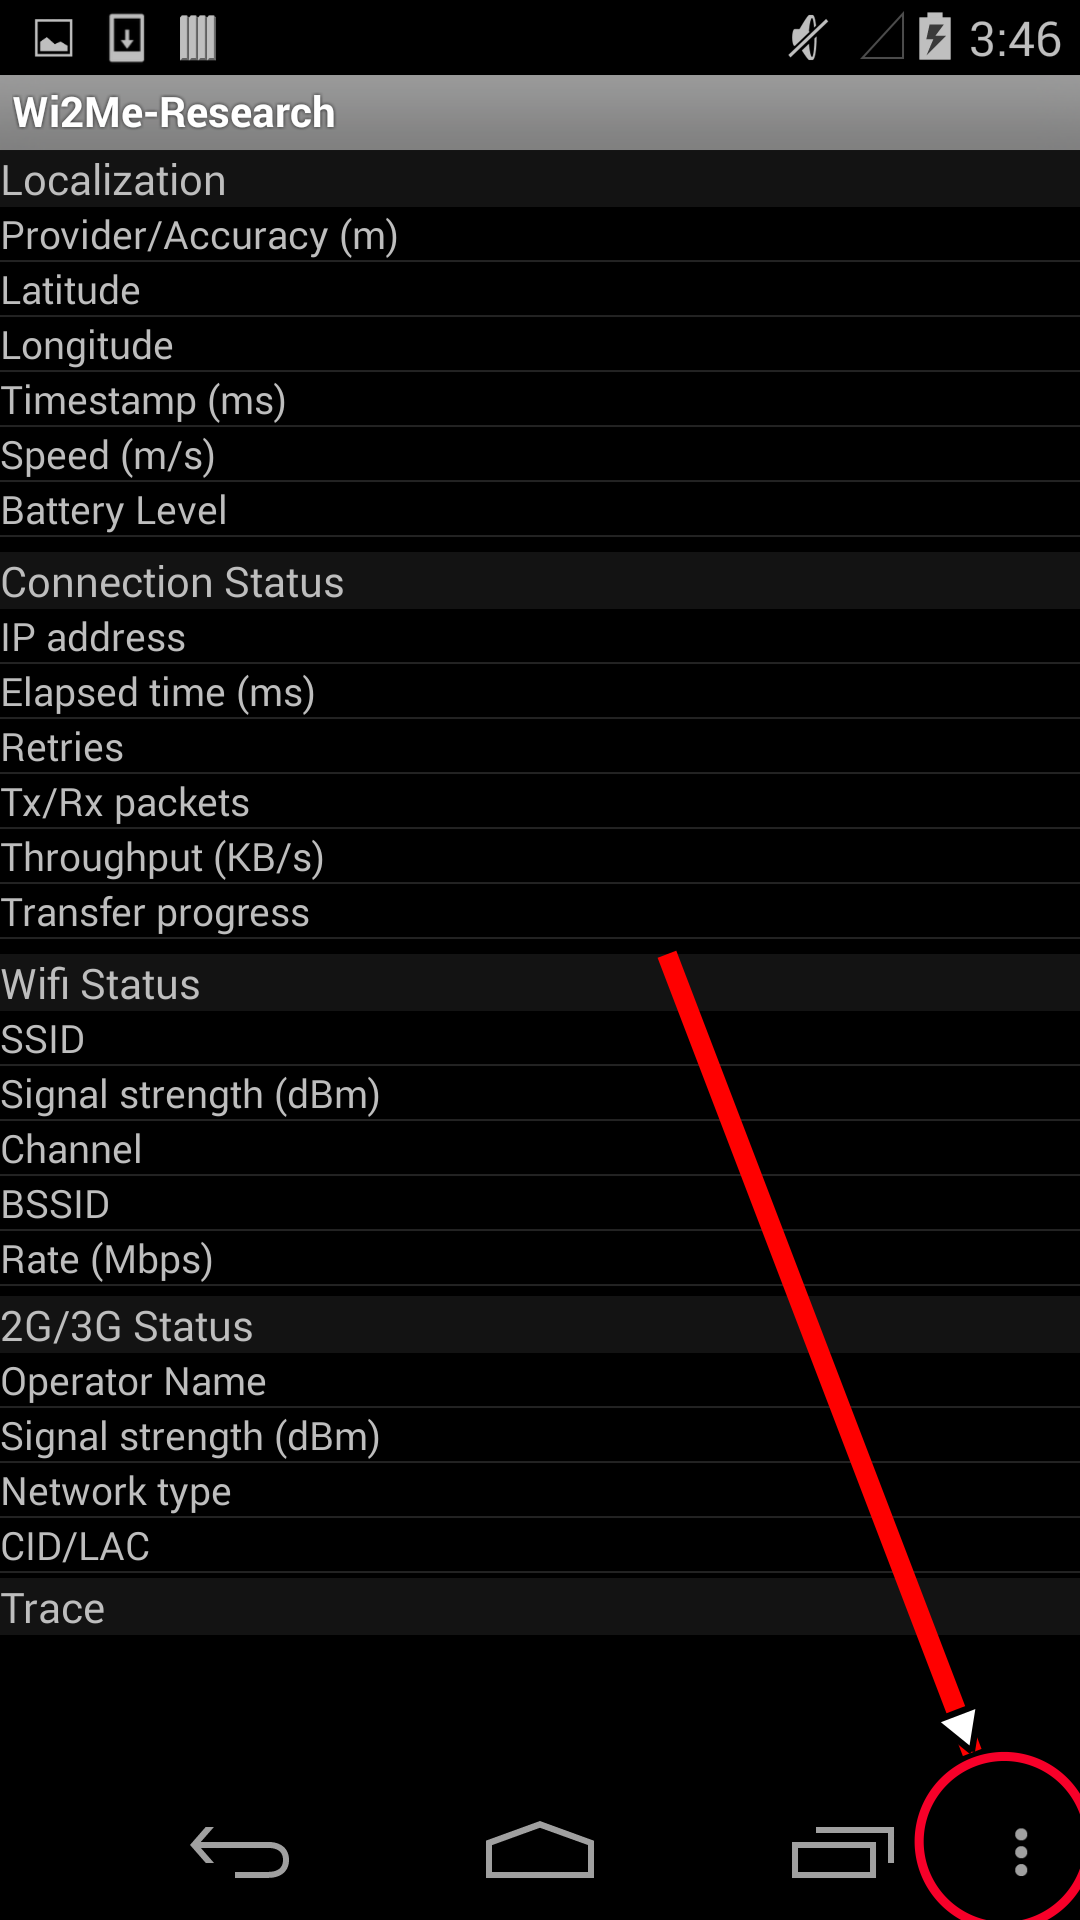
\includegraphics[height=0.4\textheight]{MenuStart.png}
\end{SCfigure}


\begin{SCfigure}[\sidecaptionrelwidth][!h]
  \centering
  \caption{\mtext{Déclencher les mesures en appuyant sur le bouton Start. Le menu va se fermer et certaines données commenceront à s'afficher à l'écran. L'écran peut maintenant être éteint.}{Trigger the mesurements by pressing the start button in the menu. The overlay menu will close and some information will start being displayed on screen. The phone's screen can now be turned off to save battery.}}
  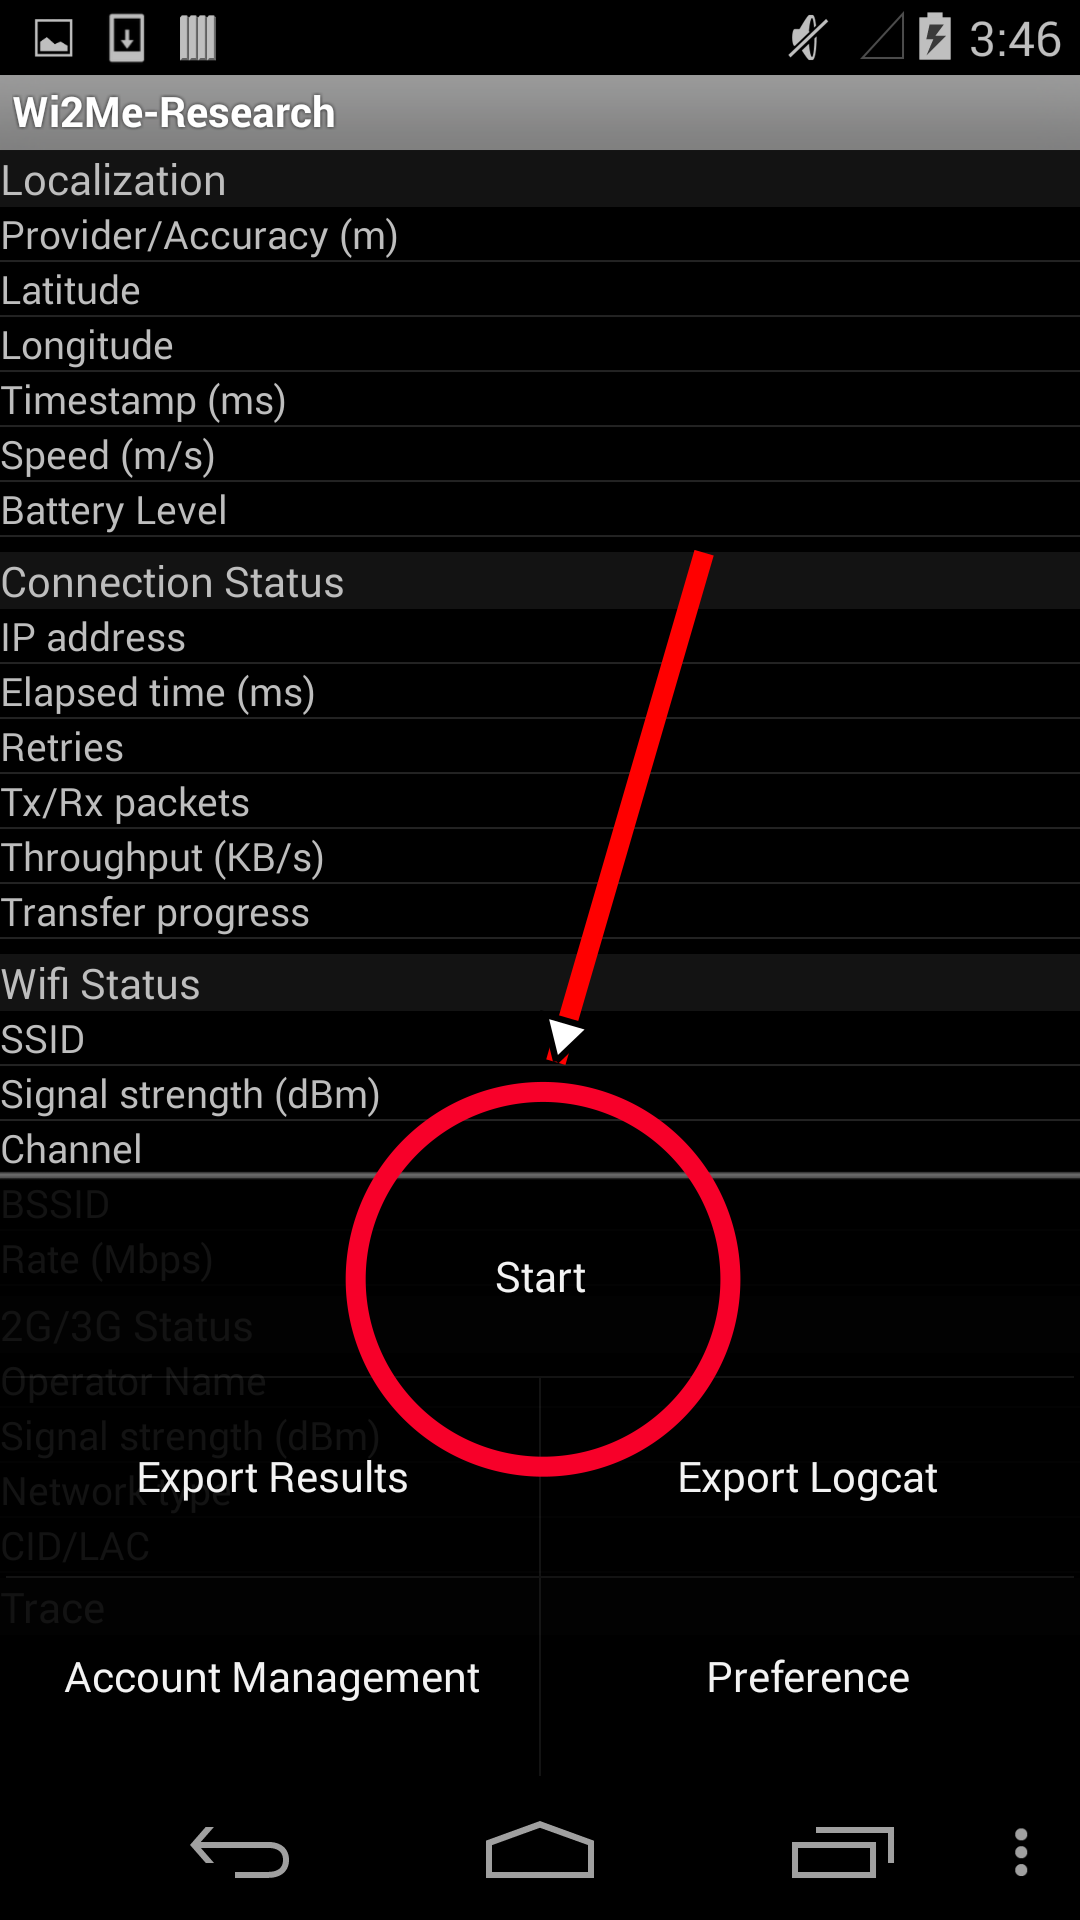
\includegraphics[height=0.4\textheight]{start.png}
\end{SCfigure}
\clearpage

%------------------------------------------------
\question{\mtext{Arrêter wi2me}{Stopping Wi2Me}}\label{stopping}

\begin{SCfigure}[\sidecaptionrelwidth][!h]
  \centering
  \caption{\mtext{ Ouvrir le menu de wi2me en utilisant le menu en bas à gauche (ou le bouton menu physique s'il existe)}{Open the application menu by using the menu button in the bottom left (or your phone's physical menu button if it exists).}}
  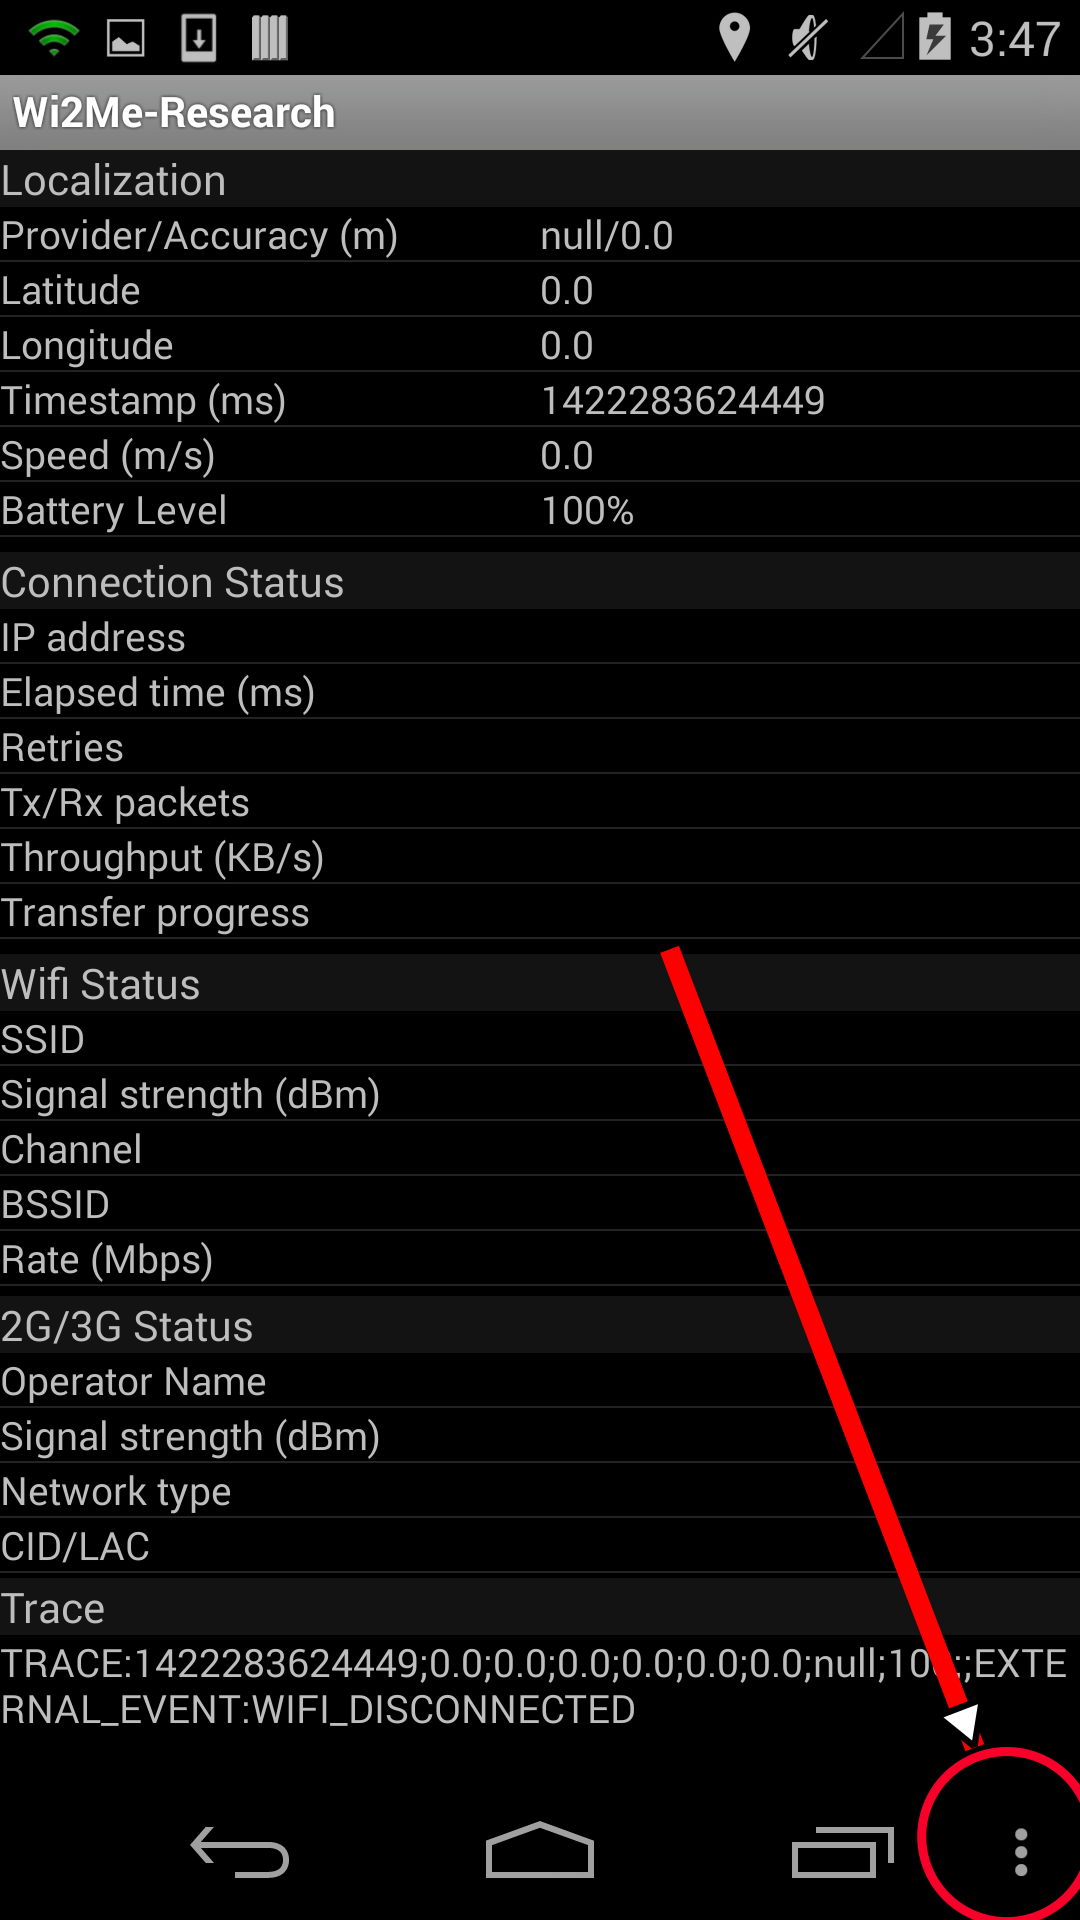
\includegraphics[height=0.4\textheight]{MenuStop.png}
\end{SCfigure}

\begin{SCfigure}[\sidecaptionrelwidth][!h]
  \centering
  \caption{\mtext{Presser le bouton stop. Après un cours moment, les données ne seront plus affichées dans l'application, qui pourra être fermée ou réduite.}{Press the stop button. After some processing, the application will stop diplaying data and can be closed or reduced.}}
  \includegraphics[height=0.4\textheight]{stop.png}
\end{SCfigure}

\question{\mtext{NOTIMPL}{exporting results}}\label{exporting}


\begin{SCfigure}[\sidecaptionrelwidth][!h]
  \centering
  \caption{
\mtext{}{After a data gathering phase, you will need to export your results for further processing. To do so, open the menu again, and press the 'export results' button. A pop up will appear asking the type of export you wish to use. Select the "Export to" SD option.
Once this is done, you can find your databases at the phone's sdcard root, under the name TraceLog\_XXXX where XXXX is the timestamp of the moment you performed the export
}
}
  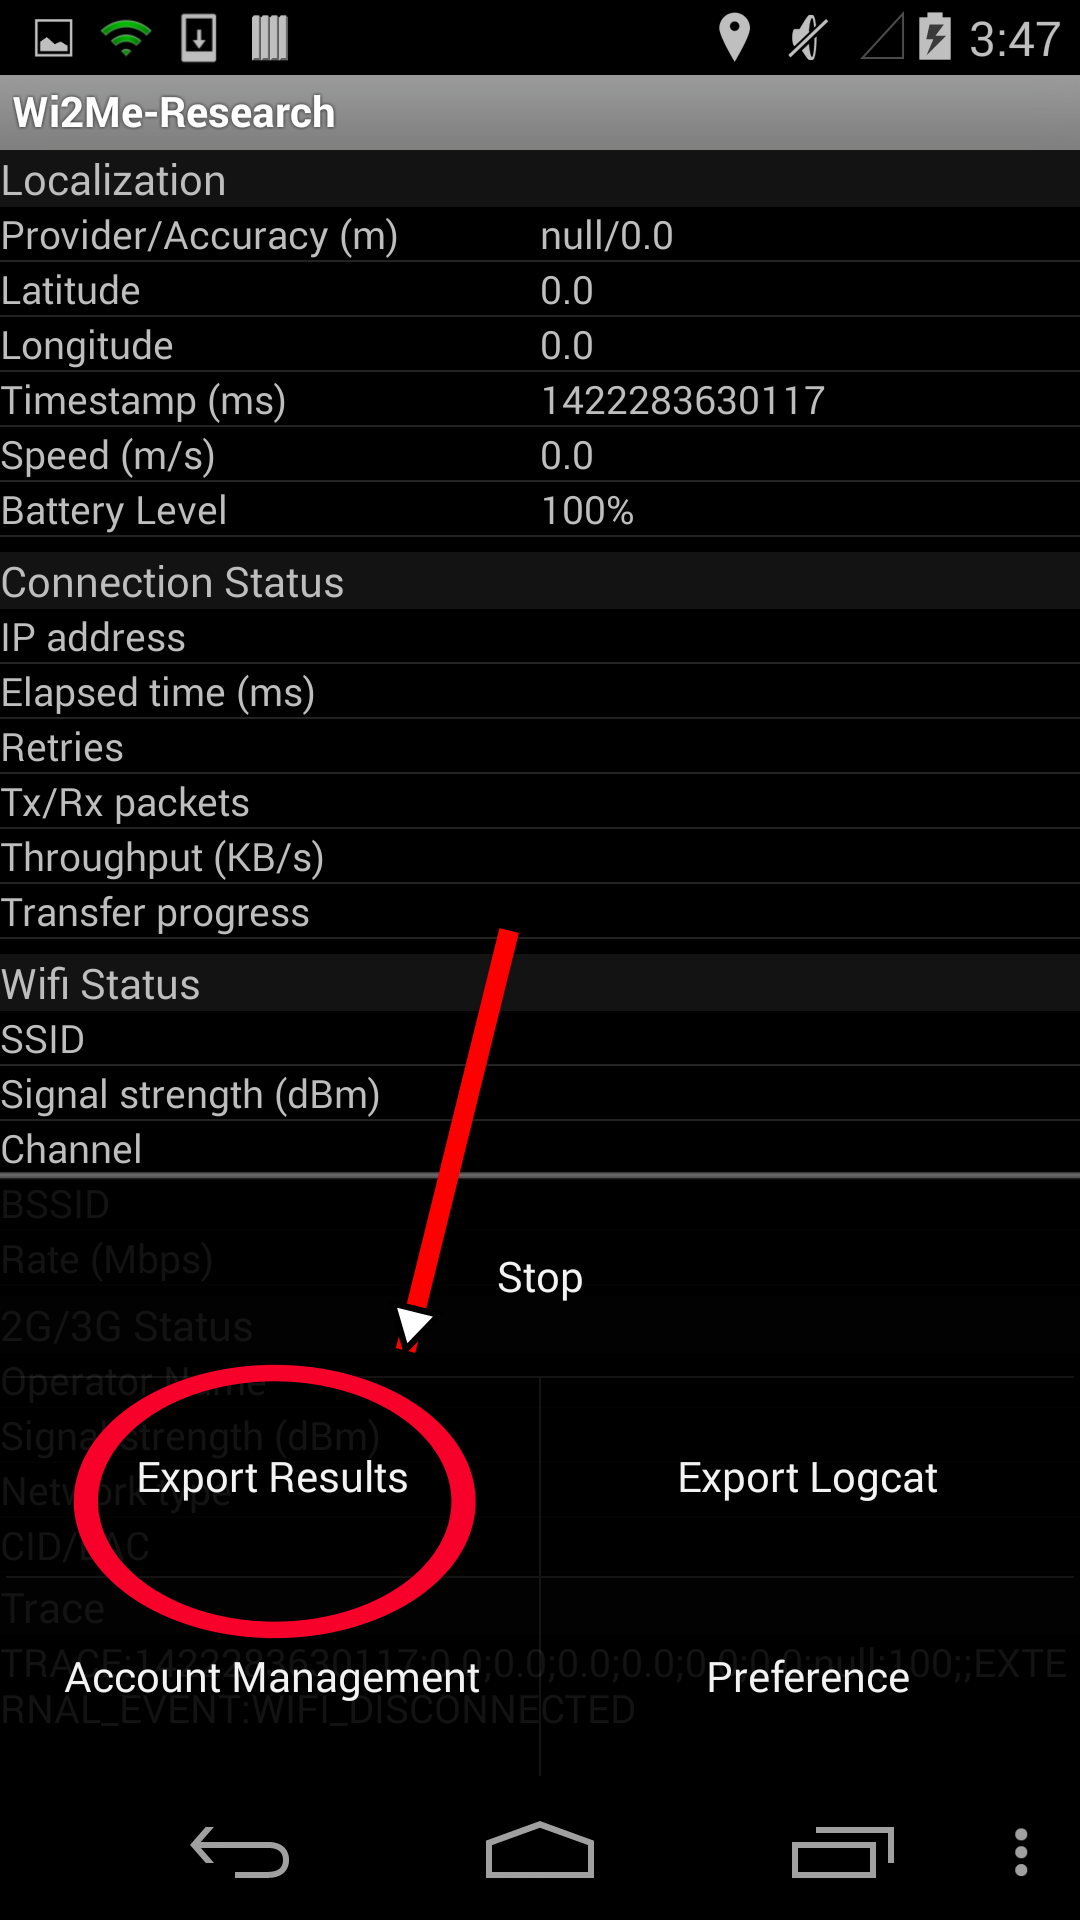
\includegraphics[height=0.4\textheight]{export.png}
\end{SCfigure}


\end{document}
